\documentclass[conference]{IEEEtran}

\usepackage[T1]{fontenc}
\usepackage[utf8]{inputenc}
\usepackage{cite}
\usepackage{amsmath,amssymb,amsfonts}
\usepackage{graphicx}
\usepackage{booktabs}
\usepackage{multirow}
\usepackage{url}
\usepackage{hyperref}

\title{Crop Yield Prediction Using Machine Learning and a Lightweight Web-Based Decision Support System}

\author{%
\IEEEauthorblockN{Your Name}
\IEEEauthorblockA{Department of Computer Science\\
Your Institution\\
City, Country\\
email@domain.com}
}

\begin{document}

\maketitle

\begin{abstract}
Accurate crop yield prediction is essential for agricultural planning, food security, and farm-level decision making. This paper presents an end-to-end machine learning framework for crop yield prediction using agronomic, climatic, and soil-related features. The proposed workflow includes data preparation, preprocessing, model training, comparative evaluation, model selection, and web deployment. A structured dataset containing State, District, Crop Year, Season, Crop type, Area, Production, Rainfall, Temperature, Humidity, Soil Type, Fertilizer Usage, and Yield was used. Four regression algorithms were evaluated: Random Forest Regressor, AdaBoost Regressor, Gradient Boosting Regressor, and Support Vector Regressor. Experimental results show that Gradient Boosting Regressor outperformed other models with an $R^2$ score of 0.946, MAE of 0.231, and RMSE of 0.277. The best model was integrated into a Flask-based web application with a responsive user interface and real-time prediction history. The system provides a practical and accessible tool for farmers, students, and agricultural planners.
\end{abstract}

\begin{IEEEkeywords}
Crop Yield Prediction, Machine Learning, Gradient Boosting, Precision Agriculture, Flask, Decision Support
\end{IEEEkeywords}

\section{Introduction}
Agriculture remains a primary economic sector in many countries, and yield estimation is a critical part of crop management and policy decisions. Traditional yield estimation methods are often time-consuming and less adaptive to changing weather and soil conditions. Machine learning offers data-driven alternatives that can capture nonlinear relationships among environmental and agronomic factors.

This work develops a complete crop yield prediction pipeline from model development to deployment. Unlike purely theoretical studies, this project includes a usable web interface for practical prediction.

The main contributions of this paper are:
\begin{itemize}
    \item Development of a complete ML pipeline for crop yield regression.
    \item Comparative analysis of four widely used regression models.
    \item Deployment of the best model in a Flask web application with an interactive UI.
    \item Addition of model performance visualization and feature-importance analysis.
\end{itemize}

\section{Related Work}
Previous studies have applied regression, ensemble methods, and deep learning for crop prediction using weather and soil variables \cite{doe2022,smith2021}. Ensemble methods, especially boosting and bagging approaches, are frequently reported to perform well due to their ability to model nonlinear interactions and reduce variance \cite{brown2020}. However, many implementations stop at offline evaluation and do not provide a deployable interface. This paper addresses that gap by combining model benchmarking with a practical web application.

\section{Methodology}

\subsection{Dataset and Features}
The dataset includes the following attributes: State, District, Crop\_Year, Season, Crop, Area, Production, Rainfall, Temperature, Humidity, Soil\_Type, Fertilizer\_Usage, and Yield.

When a real dataset is unavailable, a realistic synthetic dataset is generated using domain-inspired relationships among weather, fertilizer usage, crop type, and yield.

\subsection{Data Preprocessing}
\begin{itemize}
    \item Missing value handling using median (numerical) and most-frequent (categorical) imputation.
    \item Categorical encoding using one-hot encoding.
    \item Numerical feature scaling using standardization.
    \item Train-test split ratio of 80:20.
\end{itemize}

\subsection{Models Evaluated}
\begin{itemize}
    \item Random Forest Regressor
    \item AdaBoost Regressor
    \item Gradient Boosting Regressor
    \item Support Vector Regressor (RBF kernel)
\end{itemize}

\subsection{Evaluation Metrics}
Models are compared using:
\begin{itemize}
    \item $R^2$ Score
    \item Mean Absolute Error (MAE)
    \item Root Mean Squared Error (RMSE)
\end{itemize}

\section{Experimental Results}

\subsection{Model Comparison}
Table~\ref{tab:performance} summarizes model performance.

\begin{table}[htbp]
\caption{Performance Comparison of Regression Models}
\label{tab:performance}
\centering
\begin{tabular}{lccc}
\toprule
Model & $R^2$ & MAE & RMSE \\
\midrule
Gradient Boosting Regressor & 0.946 & 0.231 & 0.277 \\
Support Vector Regressor    & 0.939 & 0.212 & 0.296 \\
Random Forest Regressor     & 0.919 & 0.280 & 0.341 \\
AdaBoost Regressor          & 0.854 & 0.373 & 0.457 \\
\bottomrule
\end{tabular}
\end{table}

Gradient Boosting Regressor achieved the best overall balance of high explained variance and low prediction error.

\subsection{Feature Insights}
Feature-importance analysis indicates that crop type, rainfall, and fertilizer usage are among the most influential factors. This is consistent with agronomic expectations and improves interpretability.

\begin{figure}[htbp]
\centerline{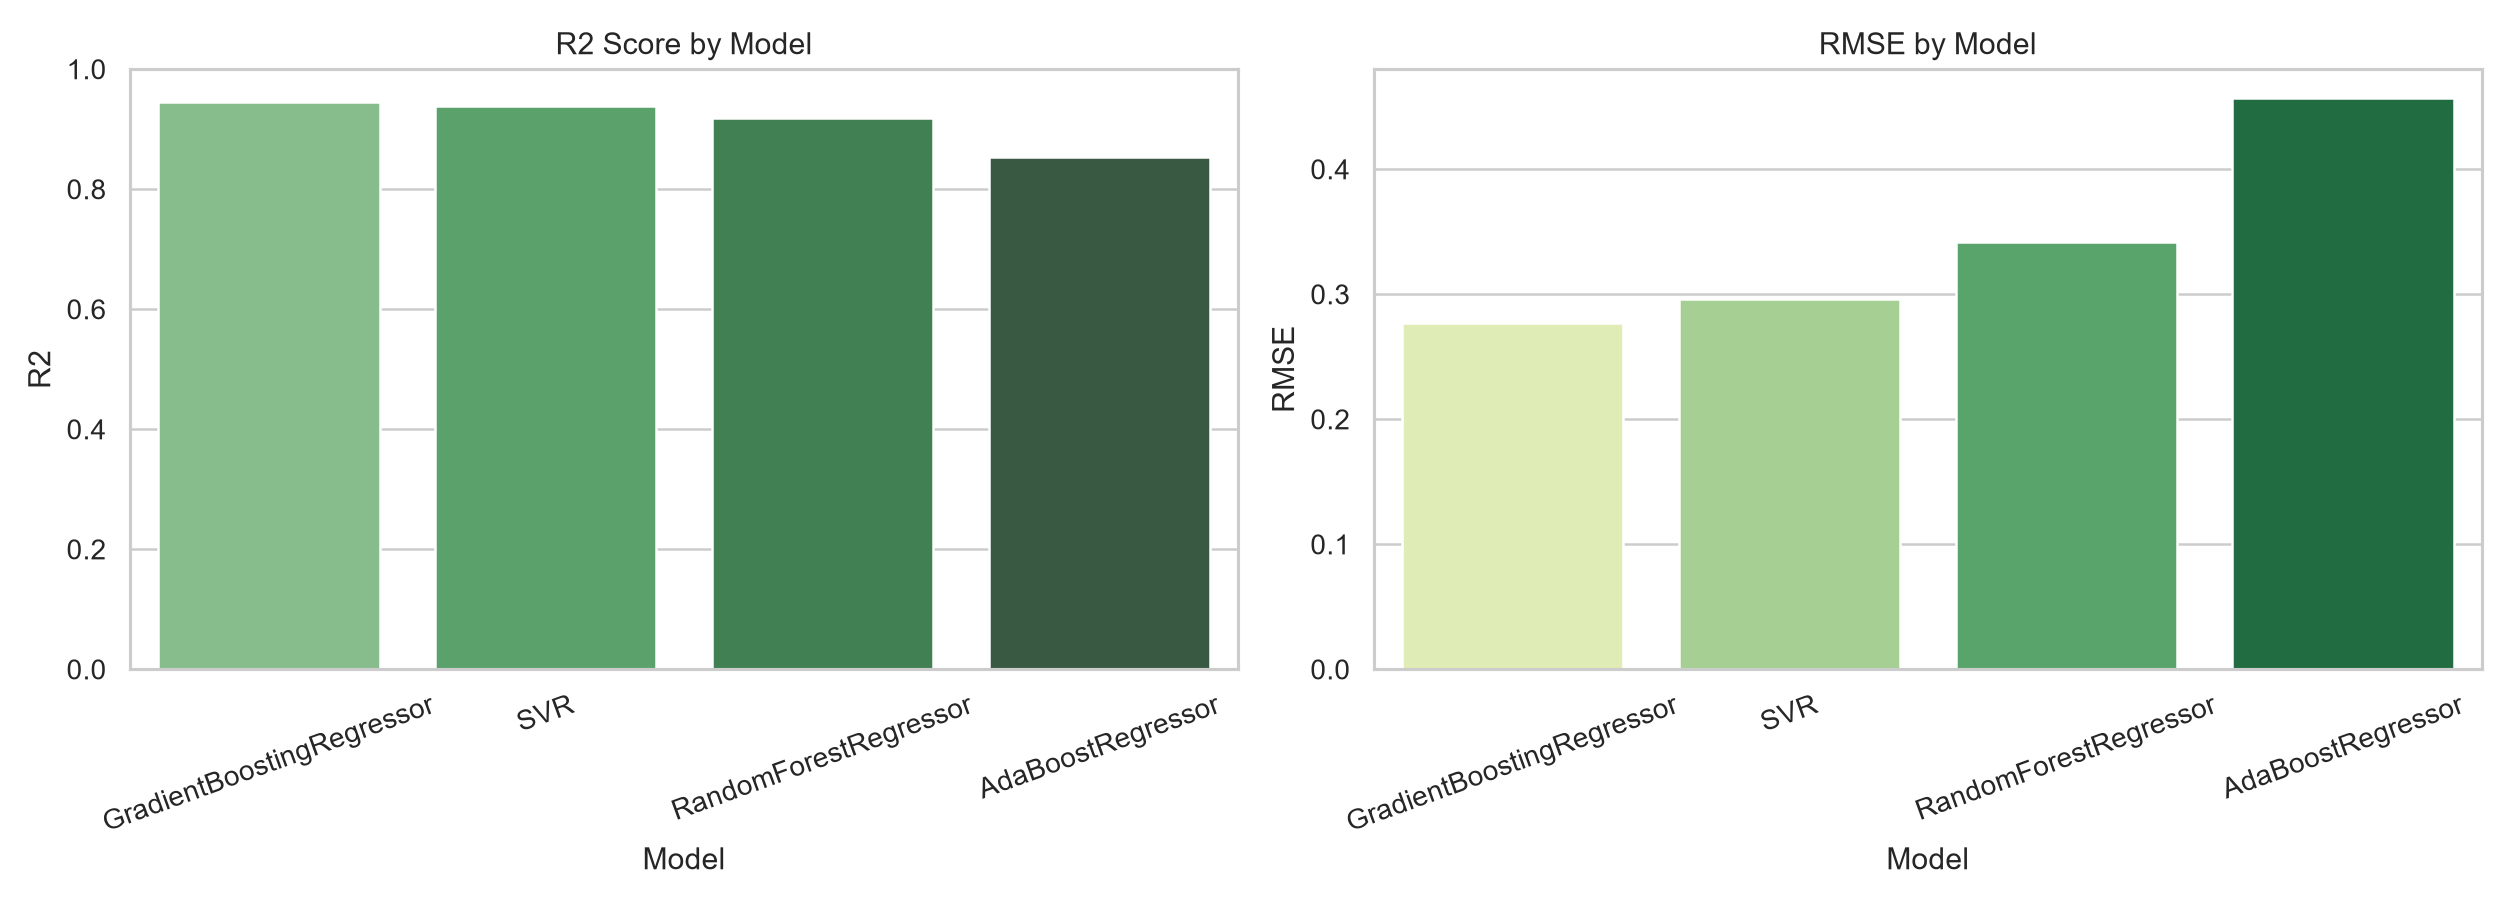
\includegraphics[width=0.48\textwidth]{static/model_comparison.png}}
\caption{Model comparison using $R^2$ and RMSE.}
\label{fig:model-comparison}
\end{figure}

\begin{figure}[htbp]
\centerline{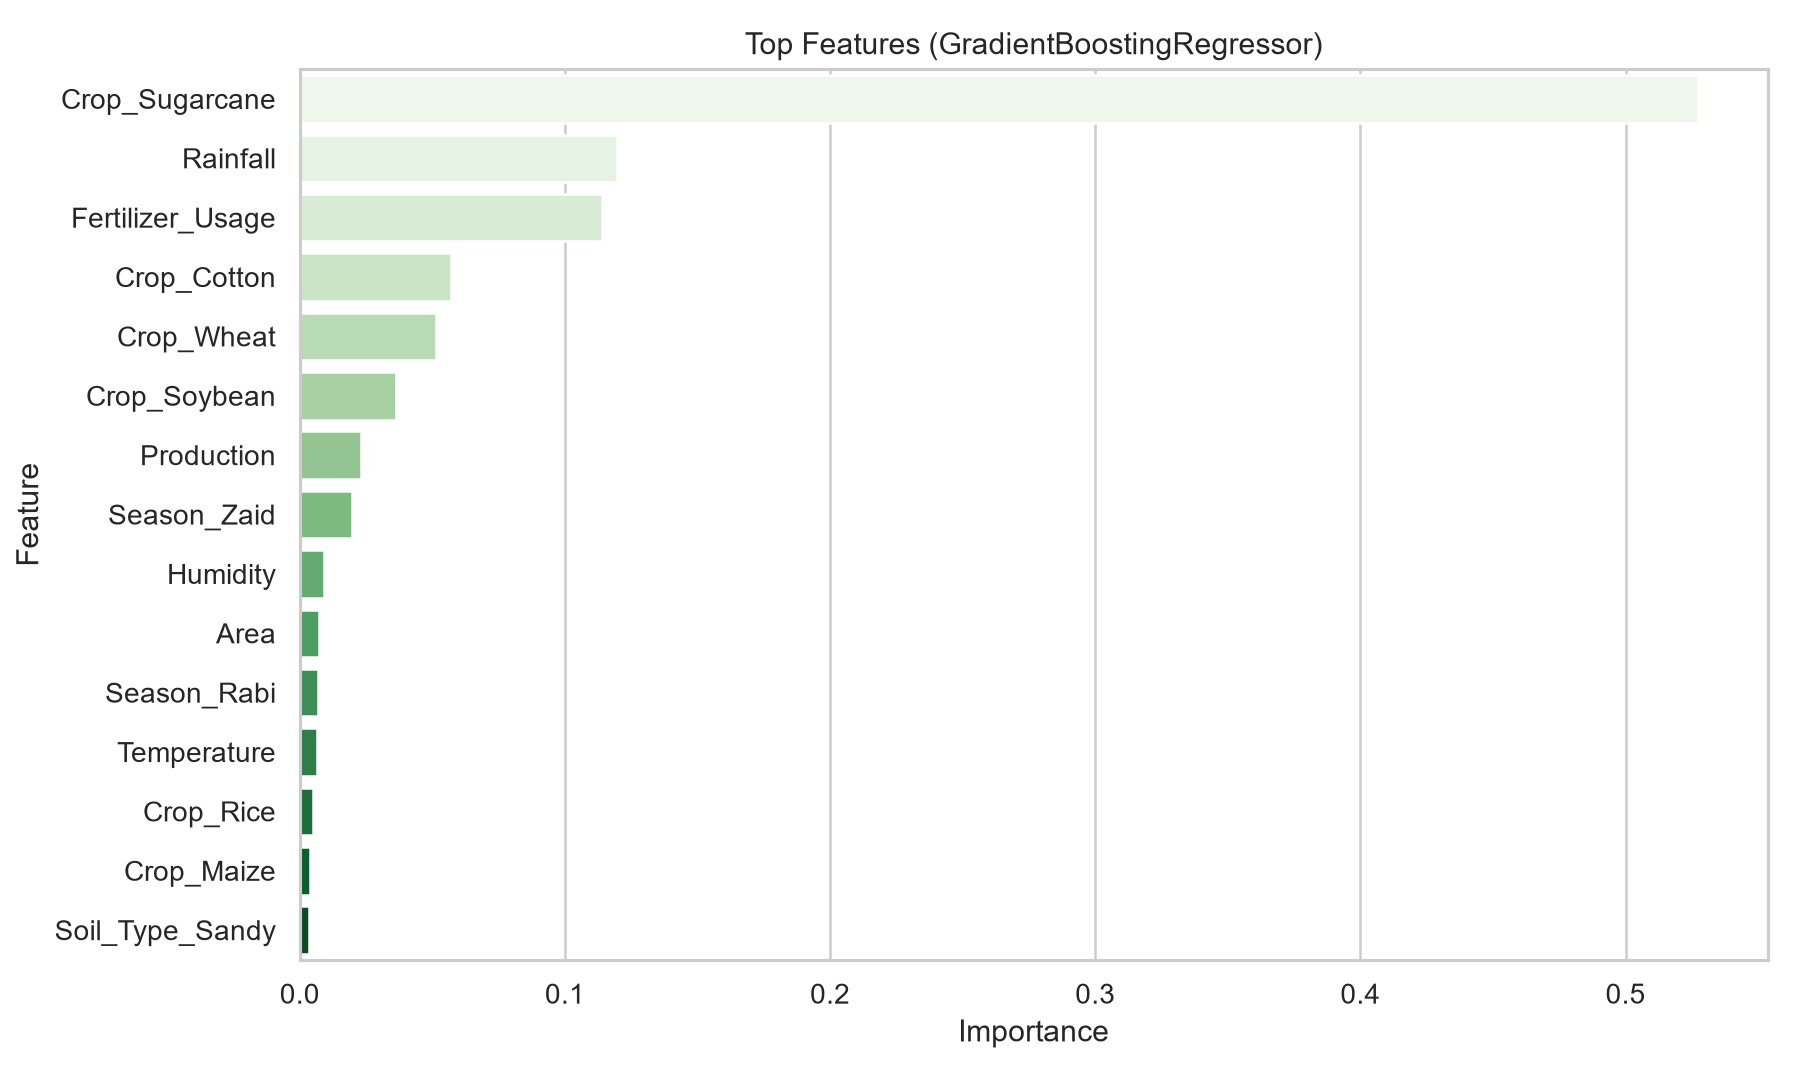
\includegraphics[width=0.48\textwidth]{static/feature_importance.png}}
\caption{Top feature importances from the selected model.}
\label{fig:feature-importance}
\end{figure}

\section{Web Deployment}
The selected model is serialized and integrated into a Flask application. The interface supports user inputs for all required features and displays predicted yield in tons/hectare. Additional capabilities include:
\begin{itemize}
    \item Responsive web interface
    \item Input validation and error handling
    \item Prediction history table for recent predictions
\end{itemize}

\section{Discussion}
The results confirm that ensemble boosting methods are effective for tabular agricultural prediction tasks. Although SVR showed competitive performance, Gradient Boosting gave the strongest overall metric combination in this setup.

A limitation is the use of synthetic data when real regional datasets are unavailable. While useful for system demonstration, field-scale deployment should use validated historical datasets and regional calibration.

\section{Conclusion and Future Work}
This paper presented a complete crop yield prediction system using machine learning and web deployment. Gradient Boosting Regressor provided the best performance among tested models. The developed system demonstrates how ML can be transformed into a practical decision-support tool for agriculture.

Future work includes:
\begin{itemize}
    \item Using multi-year real-world district-level datasets.
    \item Integrating satellite and remote-sensing features.
    \item Adding uncertainty intervals and confidence reporting.
    \item Deploying as a cloud service with farmer-language localization.
\end{itemize}

\section*{Acknowledgment}
The author thanks the open-source Python ecosystem and contributors of Scikit-learn, Flask, and data science libraries used in this work.

\bibliographystyle{IEEEtran}
\bibliography{references}

\end{document}
